\section{Threadparallelismus}
	\subsection{Grundlagen Multithreading}
		Rechner können nur eine bestimmte Anzahl an Threads echt-parallel ausführen. Um dennoch "unendlich" viele Threads unterstützen zu können und es dem Benutzer gegenüber so aussehen zu lassen, als würden diese parallel ausgeführt werden, wird in schnellen Abständen zwischen den aktiven Threads gewechselt.
		\subsubsection{Zeitscheiben Multithreading}
			Jeder Thread bekommt immer eine fixe Zeit, die er aktiv rechnen darf, bevor er wieder ausgewechselt wird (z.B. alle 50ms wird gewechselt). Die CPU muss hierfür einen Hardwaretimer besitzen. Das Betriebsystem setzt den Hardwaretimer, lässt den Thread an die CPU, und nach Ablauf der Zeit wechselt die CPU automatisch durch ein sogenanntes Interruptsignal (Unterbrechungssignal) zum Betriebssystem zurück
		\subsection{Ereignisgesteuertes Multithreading}
			Zwischen Threads wird dann gewechselt, wenn ein aktiver Thread beginnt, auf ein externes Ereignis zu warten (z.B. Antwort von der Festplatte oder Benutzereingabe). Derartige Events benötigen in der Regel ohnehin Kommunikation mit dem Betriebssystem (d.h. einen Sprung in den Betriebssystemcode), weshalb die CPU hier keine besondere Hardwareeigenschaften benötigt. Sobald das Betriebssystem wieder selbst "in der CPU" ist, kann es auch entscheiden, ob ein Threadwechsel stattfindet \newline \newline
			Ein Threadwechsel ist dabei teuer: Bei jedem Wechsel müssen die Register des Threads gesichert (und wiederhergestellt) werden, und der komplette Cacheinhalt wird in der Regel nutzlos (da der nächste Thread selten die Daten des vorherigen Threads braucht). Zeitscheiben sollten daher nicht zu niedrig gesetzt werden
	\subsection{Cachehirachie}
		Bei Multicoresystemen wird der Cache in der Regel in mehrere Hierarchiestufen unterteilt. Die folgende Grafik zeigt einen beispielhaften Aufbau für eine 4-Kern-CPU (Quadcore): \newline
		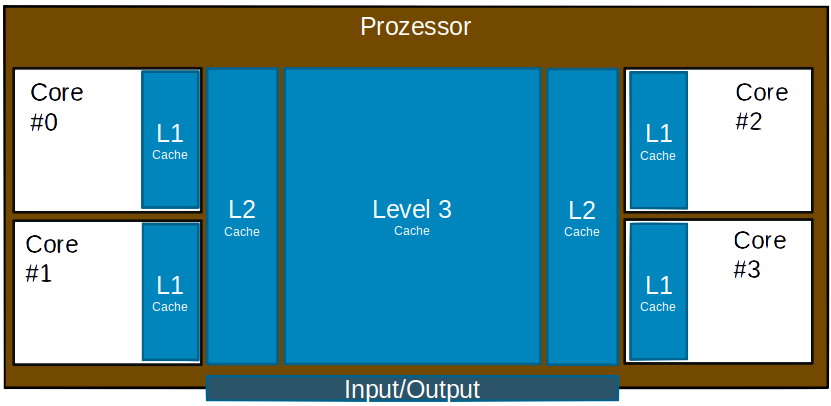
\includegraphics[scale=0.42]{quadcore.png}
	\subsection{Simultanes Multithreading}
		Bei simultanem Multithreading (SMT) nutzen wir die Tatsache aus, dass ein Thread in der Regel nicht alle Teile des Rechenwerks (und theoretisch auch nicht den ganzen Cache) gleichzeitig benötigt und erweitern den Kern daher um ein weiteres Frontend, einen weiteren Registersatz und einen weiteren Befehlszähler. Das Rechenwerk bleibt unverändert. Diese Änderungen sind deutlich günstiger, als den kompletten Kern zu verdoppeln \newline \newline
		Dadurch ist es bei SMT möglich, zwei Thread echt-parallel im selben Kern auszuführen. Dies klappt jedoch nur, wenn die Threads unterschiedliche Operationen ausführen wollen, z.B.: Thread 1 möchte addieren, während Thread 2 dividiert \newline \newline
		Bei einem physischen CPU Kern, der durch 2-fachem SMT bis zu 2 Threads gleichzeitig ausführen kann, spricht man dann auch davon, dass er aus 2 logischen Kernen besteht
		
